\documentclass[tikz,border=3pt]{standalone}
\usepackage{amsmath}
\usetikzlibrary{arrows.meta,patterns,decorations.pathreplacing}
\definecolor{ohred}{HTML}{B23B2E}
\definecolor{rcblue}{HTML}{2F5FA6}
\tikzset{
  meshup/.style={fill=black!18, fill opacity=0.22, draw=black!35, draw opacity=0.45, line width=0.22pt},
  meshdown/.style={fill=black!28, fill opacity=0.22, draw=black!38, draw opacity=0.45, line width=0.22pt},
  meshside/.style={fill=black!10, fill opacity=0.18, draw=black!32, draw opacity=0.45, line width=0.22pt},
  srcface/.style={fill=ohred!45, fill opacity=0.72, draw=ohred!85!black, draw opacity=0.96, line width=0.9pt},
  recface/.style={fill=rcblue!42, fill opacity=0.72, draw=rcblue!85!black, draw opacity=0.96, line width=0.9pt},
  plate/.style={fill=black!4, fill opacity=0.22, draw=black!35, draw opacity=0.55, line width=0.5pt, pattern=north east lines, pattern color=black!25},
  ray/.style={->, >=Latex, dash pattern=on 2.2pt off 2.2pt, line width=1.0pt, black!70},
  axis/.style={->, >=Latex, line width=1.2pt, black!70},
  normSrc/.style={->, >=Latex, line width=1.1pt, ohred!80!black},
  normRec/.style={->, >=Latex, line width=1.1pt, rcblue!82!black},
  measure/.style={<->, >=Latex, line width=0.65pt, black!55},
  srcDot/.style={ohred!80!black},
  recDot/.style={rcblue!82!black},
  groundDot/.style={rcblue!82!black},
  termLabel/.style={font=\small\bfseries, text=black!80, align=center},
  panelLabel/.style={font=\bfseries, text=black!80},
}
\begin{document}
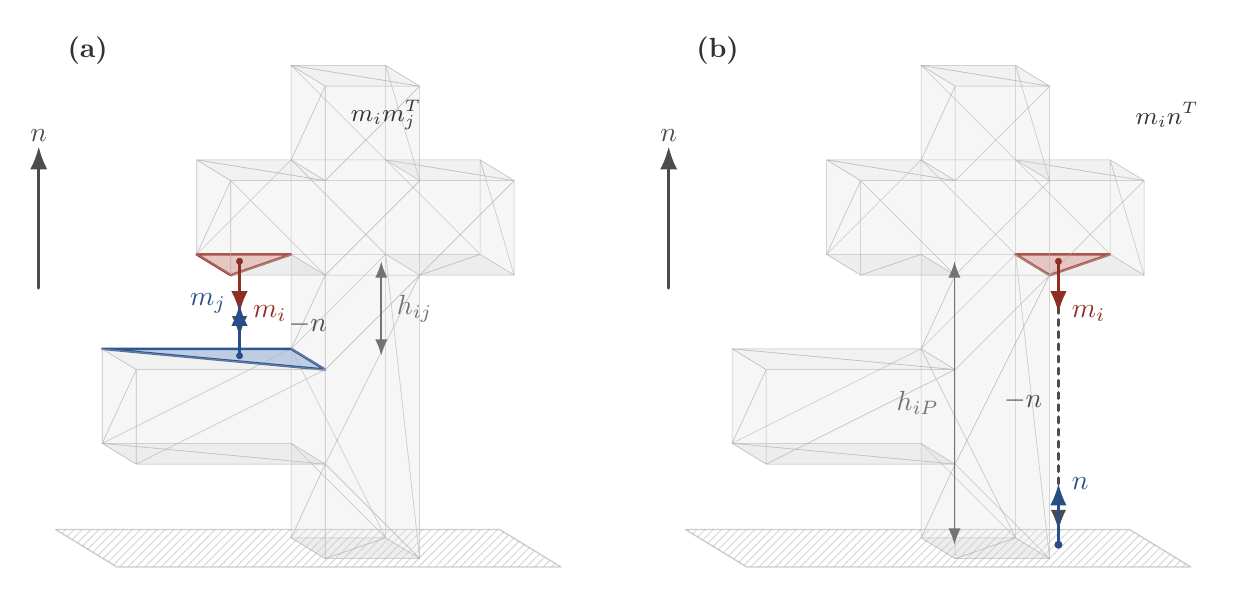
\begin{tikzpicture}[line join=round,line cap=round]
\begin{scope}
\node[panelLabel] at (-2.8,6.7) {(a)};
\filldraw[plate] (-3.209,0.620) -- (2.431,0.620) -- (3.209,0.144) -- (-2.431,0.144) -- cycle;
\filldraw[meshside] (-2.616,1.714) -- (-0.216,1.714) -- (-0.216,2.914) -- cycle;
\filldraw[meshside] (-2.616,1.714) -- (-0.216,2.914) -- (-2.616,2.914) -- cycle;
\filldraw[meshside] (-1.416,4.114) -- (-0.216,4.114) -- (-0.216,5.314) -- cycle;
\filldraw[meshside] (-1.416,4.114) -- (-0.216,5.314) -- (-1.416,5.314) -- cycle;
\filldraw[meshside] (-0.216,4.114) -- (-0.216,2.914) -- (0.984,4.114) -- cycle;
\filldraw[meshside] (0.984,0.514) -- (0.984,4.114) -- (-0.216,2.914) -- cycle;
\filldraw[meshside] (-0.216,1.714) -- (0.984,0.514) -- (-0.216,2.914) -- cycle;
\filldraw[meshside] (-0.216,0.514) -- (0.984,0.514) -- (-0.216,1.714) -- cycle;
\filldraw[meshside] (-0.216,5.314) -- (-0.216,4.114) -- (0.984,4.114) -- cycle;
\filldraw[meshside] (0.984,4.114) -- (0.984,5.314) -- (-0.216,5.314) -- cycle;
\filldraw[meshside] (-0.216,6.514) -- (-0.216,5.314) -- (0.984,5.314) -- cycle;
\filldraw[meshside] (-0.216,6.514) -- (0.984,5.314) -- (0.984,6.514) -- cycle;
\filldraw[meshside] (0.984,5.314) -- (0.984,4.114) -- (2.184,4.114) -- cycle;
\filldraw[meshside] (0.984,5.314) -- (2.184,4.114) -- (2.184,5.314) -- cycle;
\filldraw[meshdown] (-0.216,1.714) -- (-2.616,1.714) -- (0.216,1.450) -- cycle;
\filldraw[recface] (-2.616,2.914) -- (-0.216,2.914) -- (0.216,2.650) -- cycle;
\filldraw[srcface] (-0.984,3.850) -- (-0.216,4.114) -- (-1.416,4.114) -- cycle;
\filldraw[meshside] (-2.184,2.650) -- (-2.616,1.714) -- (-2.616,2.914) -- cycle;
\filldraw[meshup] (-1.416,5.314) -- (-0.216,5.314) -- (0.216,5.050) -- cycle;
\filldraw[meshside] (-0.984,5.050) -- (-1.416,4.114) -- (-1.416,5.314) -- cycle;
\filldraw[meshside] (0.216,3.850) -- (-0.216,2.914) -- (-0.216,4.114) -- cycle;
\filldraw[meshside] (0.216,1.450) -- (-0.216,0.514) -- (-0.216,1.714) -- cycle;
\filldraw[meshside] (0.216,6.250) -- (-0.216,5.314) -- (-0.216,6.514) -- cycle;
\filldraw[meshdown] (1.416,3.850) -- (2.184,4.114) -- (0.984,4.114) -- cycle;
\filldraw[meshup] (0.984,5.314) -- (2.184,5.314) -- (2.616,5.050) -- cycle;
\filldraw[meshside] (0.984,6.514) -- (0.984,5.314) -- (1.416,5.050) -- cycle;
\filldraw[meshup] (-0.216,6.514) -- (0.984,6.514) -- (1.416,6.250) -- cycle;
\filldraw[meshdown] (0.216,0.250) -- (0.984,0.514) -- (-0.216,0.514) -- cycle;
\filldraw[meshside] (2.184,5.314) -- (2.184,4.114) -- (2.616,3.850) -- cycle;
\filldraw[meshside] (0.984,4.114) -- (0.984,0.514) -- (1.416,0.250) -- cycle;
\filldraw[meshdown] (-2.184,1.450) -- (0.216,1.450) -- (-2.616,1.714) -- cycle;
\filldraw[meshup] (-2.616,2.914) -- (0.216,2.650) -- (-2.184,2.650) -- cycle;
\filldraw[meshdown] (-0.984,3.850) -- (0.216,3.850) -- (-0.216,4.114) -- cycle;
\filldraw[meshside] (-2.184,2.650) -- (-2.184,1.450) -- (-2.616,1.714) -- cycle;
\filldraw[meshup] (-1.416,5.314) -- (0.216,5.050) -- (-0.984,5.050) -- cycle;
\filldraw[meshside] (-0.984,5.050) -- (-0.984,3.850) -- (-1.416,4.114) -- cycle;
\filldraw[meshside] (0.216,3.850) -- (0.216,2.650) -- (-0.216,2.914) -- cycle;
\filldraw[meshside] (0.216,1.450) -- (0.216,0.250) -- (-0.216,0.514) -- cycle;
\filldraw[meshside] (0.216,6.250) -- (0.216,5.050) -- (-0.216,5.314) -- cycle;
\filldraw[meshdown] (1.416,3.850) -- (2.616,3.850) -- (2.184,4.114) -- cycle;
\filldraw[meshup] (0.984,5.314) -- (2.616,5.050) -- (1.416,5.050) -- cycle;
\filldraw[meshside] (0.984,6.514) -- (1.416,5.050) -- (1.416,6.250) -- cycle;
\filldraw[meshup] (-0.216,6.514) -- (1.416,6.250) -- (0.216,6.250) -- cycle;
\filldraw[meshdown] (0.216,0.250) -- (1.416,0.250) -- (0.984,0.514) -- cycle;
\filldraw[meshside] (2.184,5.314) -- (2.616,3.850) -- (2.616,5.050) -- cycle;
\filldraw[meshside] (0.984,4.114) -- (1.416,0.250) -- (1.416,3.850) -- cycle;
\filldraw[meshside] (0.216,2.650) -- (0.216,1.450) -- (-2.184,1.450) -- cycle;
\filldraw[meshside] (-2.184,2.650) -- (0.216,2.650) -- (-2.184,1.450) -- cycle;
\filldraw[meshside] (-0.984,5.050) -- (0.216,5.050) -- (0.216,3.850) -- cycle;
\filldraw[meshside] (-0.984,5.050) -- (0.216,3.850) -- (-0.984,3.850) -- cycle;
\filldraw[meshside] (1.416,3.850) -- (1.416,5.050) -- (2.616,5.050) -- cycle;
\filldraw[meshside] (1.416,3.850) -- (2.616,5.050) -- (2.616,3.850) -- cycle;
\filldraw[meshside] (1.416,3.850) -- (1.416,0.250) -- (0.216,1.450) -- cycle;
\filldraw[meshside] (0.216,0.250) -- (0.216,1.450) -- (1.416,0.250) -- cycle;
\filldraw[meshside] (0.216,1.450) -- (0.216,2.650) -- (1.416,3.850) -- cycle;
\filldraw[meshside] (0.216,2.650) -- (0.216,3.850) -- (1.416,3.850) -- cycle;
\filldraw[meshside] (1.416,5.050) -- (1.416,3.850) -- (0.216,3.850) -- cycle;
\filldraw[meshside] (0.216,3.850) -- (0.216,5.050) -- (1.416,5.050) -- cycle;
\filldraw[meshside] (1.416,6.250) -- (1.416,5.050) -- (0.216,5.050) -- cycle;
\filldraw[meshside] (1.416,6.250) -- (0.216,5.050) -- (0.216,6.250) -- cycle;
\draw[ray] (-0.872,3.936) -- (-0.872,3.066) node[midway,right=14pt,yshift=-8pt]{$-n$};
\draw[normSrc] (-0.872,4.026) -- (-0.872,3.366) node[right=1pt]{$m_i$};
\draw[normRec] (-0.872,2.826) -- (-0.872,3.486) node[left=1pt]{$m_j$};
\fill[srcDot] (-0.872,4.026) circle (1.25pt);
\fill[recDot] (-0.872,2.826) circle (1.25pt);
\draw[measure] (0.928,4.026) -- (0.928,2.826) node[midway,right=2pt]{$h_{ij}$};
\node[termLabel] at (0.988,5.886) {$m_i m_j^T$};
\draw[axis] (-3.422,3.687) -- (-3.422,5.487) node[above,inner sep=1pt]{$n$};
\end{scope}
\begin{scope}[xshift=8.0cm]
\node[panelLabel] at (-2.8,6.7) {(b)};
\filldraw[plate] (-3.209,0.620) -- (2.431,0.620) -- (3.209,0.144) -- (-2.431,0.144) -- cycle;
\filldraw[meshside] (-2.616,1.714) -- (-0.216,1.714) -- (-0.216,2.914) -- cycle;
\filldraw[meshside] (-2.616,1.714) -- (-0.216,2.914) -- (-2.616,2.914) -- cycle;
\filldraw[meshside] (-1.416,4.114) -- (-0.216,4.114) -- (-0.216,5.314) -- cycle;
\filldraw[meshside] (-1.416,4.114) -- (-0.216,5.314) -- (-1.416,5.314) -- cycle;
\filldraw[meshside] (-0.216,4.114) -- (-0.216,2.914) -- (0.984,4.114) -- cycle;
\filldraw[meshside] (0.984,0.514) -- (0.984,4.114) -- (-0.216,2.914) -- cycle;
\filldraw[meshside] (-0.216,1.714) -- (0.984,0.514) -- (-0.216,2.914) -- cycle;
\filldraw[meshside] (-0.216,0.514) -- (0.984,0.514) -- (-0.216,1.714) -- cycle;
\filldraw[meshside] (-0.216,5.314) -- (-0.216,4.114) -- (0.984,4.114) -- cycle;
\filldraw[meshside] (0.984,4.114) -- (0.984,5.314) -- (-0.216,5.314) -- cycle;
\filldraw[meshside] (-0.216,6.514) -- (-0.216,5.314) -- (0.984,5.314) -- cycle;
\filldraw[meshside] (-0.216,6.514) -- (0.984,5.314) -- (0.984,6.514) -- cycle;
\filldraw[meshside] (0.984,5.314) -- (0.984,4.114) -- (2.184,4.114) -- cycle;
\filldraw[meshside] (0.984,5.314) -- (2.184,4.114) -- (2.184,5.314) -- cycle;
\filldraw[meshdown] (-0.216,1.714) -- (-2.616,1.714) -- (0.216,1.450) -- cycle;
\filldraw[meshup] (-2.616,2.914) -- (-0.216,2.914) -- (0.216,2.650) -- cycle;
\filldraw[meshdown] (-0.984,3.850) -- (-0.216,4.114) -- (-1.416,4.114) -- cycle;
\filldraw[meshside] (-2.184,2.650) -- (-2.616,1.714) -- (-2.616,2.914) -- cycle;
\filldraw[meshup] (-1.416,5.314) -- (-0.216,5.314) -- (0.216,5.050) -- cycle;
\filldraw[meshside] (-0.984,5.050) -- (-1.416,4.114) -- (-1.416,5.314) -- cycle;
\filldraw[meshside] (0.216,3.850) -- (-0.216,2.914) -- (-0.216,4.114) -- cycle;
\filldraw[meshside] (0.216,1.450) -- (-0.216,0.514) -- (-0.216,1.714) -- cycle;
\filldraw[meshside] (0.216,6.250) -- (-0.216,5.314) -- (-0.216,6.514) -- cycle;
\filldraw[srcface] (1.416,3.850) -- (2.184,4.114) -- (0.984,4.114) -- cycle;
\filldraw[meshup] (0.984,5.314) -- (2.184,5.314) -- (2.616,5.050) -- cycle;
\filldraw[meshside] (0.984,6.514) -- (0.984,5.314) -- (1.416,5.050) -- cycle;
\filldraw[meshup] (-0.216,6.514) -- (0.984,6.514) -- (1.416,6.250) -- cycle;
\filldraw[meshdown] (0.216,0.250) -- (0.984,0.514) -- (-0.216,0.514) -- cycle;
\filldraw[meshside] (2.184,5.314) -- (2.184,4.114) -- (2.616,3.850) -- cycle;
\filldraw[meshside] (0.984,4.114) -- (0.984,0.514) -- (1.416,0.250) -- cycle;
\filldraw[meshdown] (-2.184,1.450) -- (0.216,1.450) -- (-2.616,1.714) -- cycle;
\filldraw[meshup] (-2.616,2.914) -- (0.216,2.650) -- (-2.184,2.650) -- cycle;
\filldraw[meshdown] (-0.984,3.850) -- (0.216,3.850) -- (-0.216,4.114) -- cycle;
\filldraw[meshside] (-2.184,2.650) -- (-2.184,1.450) -- (-2.616,1.714) -- cycle;
\filldraw[meshup] (-1.416,5.314) -- (0.216,5.050) -- (-0.984,5.050) -- cycle;
\filldraw[meshside] (-0.984,5.050) -- (-0.984,3.850) -- (-1.416,4.114) -- cycle;
\filldraw[meshside] (0.216,3.850) -- (0.216,2.650) -- (-0.216,2.914) -- cycle;
\filldraw[meshside] (0.216,1.450) -- (0.216,0.250) -- (-0.216,0.514) -- cycle;
\filldraw[meshside] (0.216,6.250) -- (0.216,5.050) -- (-0.216,5.314) -- cycle;
\filldraw[meshdown] (1.416,3.850) -- (2.616,3.850) -- (2.184,4.114) -- cycle;
\filldraw[meshup] (0.984,5.314) -- (2.616,5.050) -- (1.416,5.050) -- cycle;
\filldraw[meshside] (0.984,6.514) -- (1.416,5.050) -- (1.416,6.250) -- cycle;
\filldraw[meshup] (-0.216,6.514) -- (1.416,6.250) -- (0.216,6.250) -- cycle;
\filldraw[meshdown] (0.216,0.250) -- (1.416,0.250) -- (0.984,0.514) -- cycle;
\filldraw[meshside] (2.184,5.314) -- (2.616,3.850) -- (2.616,5.050) -- cycle;
\filldraw[meshside] (0.984,4.114) -- (1.416,0.250) -- (1.416,3.850) -- cycle;
\filldraw[meshside] (0.216,2.650) -- (0.216,1.450) -- (-2.184,1.450) -- cycle;
\filldraw[meshside] (-2.184,2.650) -- (0.216,2.650) -- (-2.184,1.450) -- cycle;
\filldraw[meshside] (-0.984,5.050) -- (0.216,5.050) -- (0.216,3.850) -- cycle;
\filldraw[meshside] (-0.984,5.050) -- (0.216,3.850) -- (-0.984,3.850) -- cycle;
\filldraw[meshside] (1.416,3.850) -- (1.416,5.050) -- (2.616,5.050) -- cycle;
\filldraw[meshside] (1.416,3.850) -- (2.616,5.050) -- (2.616,3.850) -- cycle;
\filldraw[meshside] (1.416,3.850) -- (1.416,0.250) -- (0.216,1.450) -- cycle;
\filldraw[meshside] (0.216,0.250) -- (0.216,1.450) -- (1.416,0.250) -- cycle;
\filldraw[meshside] (0.216,1.450) -- (0.216,2.650) -- (1.416,3.850) -- cycle;
\filldraw[meshside] (0.216,2.650) -- (0.216,3.850) -- (1.416,3.850) -- cycle;
\filldraw[meshside] (1.416,5.050) -- (1.416,3.850) -- (0.216,3.850) -- cycle;
\filldraw[meshside] (0.216,3.850) -- (0.216,5.050) -- (1.416,5.050) -- cycle;
\filldraw[meshside] (1.416,6.250) -- (1.416,5.050) -- (0.216,5.050) -- cycle;
\filldraw[meshside] (1.416,6.250) -- (0.216,5.050) -- (0.216,6.250) -- cycle;
\draw[ray] (1.528,3.906) -- (1.528,0.606) node[midway,left=2pt]{$-n$};
\draw[normSrc] (1.528,4.026) -- (1.528,3.366) node[right=1pt]{$m_i$};
\fill[srcDot] (1.528,4.026) circle (1.25pt);
\fill[groundDot] (1.528,0.426) circle (1.45pt);
\draw[normRec] (1.528,0.426) -- (1.528,1.206) node[right=1pt]{$n$};
\draw[measure] (0.208,4.026) -- (0.208,0.426) node[midway,left=2pt]{$h_{iP}$};
\node[termLabel] at (2.908,5.886) {$m_i n^T$};
\draw[axis] (-3.422,3.687) -- (-3.422,5.487) node[above,inner sep=1pt]{$n$};
\end{scope}
\end{tikzpicture}
\end{document}
